\documentclass[12pt, a4paper, danish]{article}
\usepackage[danish]{babel}
\usepackage{geometry}
\usepackage{fancyhdr}
\usepackage{setspace}
\usepackage{graphicx}
\usepackage{hyperref}
\usepackage{listings}
\usepackage{xcolor}
\usepackage{tikz}

\geometry{margin=2.5cm}
\onehalfspacing
\setlength{\headheight}{14.5pt}
\pagestyle{fancy}
\fancyhead[R]{\thepage}
\fancyfoot{}

\lstset{
    language=[Sharp]C,
    basicstyle=\ttfamily\small,
    keywordstyle=\color{blue},
    commentstyle=\color{gray},
    breaklines=true,
    showstringspaces=false
}

\begin{document}

% ============================================
% FORSIDE
% ============================================
\begin{titlepage}
    \centering
    \vspace*{\fill}
    
    \Large
    \textbf{Securing Audit Logs with Hash Chains and HMAC}
    
    \vspace{0.5cm}
    Eksamen i Secure Software Development
    
    \vspace{2cm}
    \normalsize
    Projektgruppe: [Mikkel Bak Markers]
    
    \vspace{0.3cm}
    Dato: \today
    
    \vspace*{\fill}
\end{titlepage}

% ============================================
% INDHOLDSFORTEGNELSE
% ============================================
\newpage
\tableofcontents

% ============================================
% INTRODUKTION
% ============================================
\newpage
\section{Introduktion}

\subsection{Projektets Formål}
Mit mål med opgaven er, at demonstrere hvordan man kan implementere 
sikkerhedsforanstaltninger i et system der håndterer "audit logs". Fokus ligger på at sikre integritet af logs ved hjælp af hash-kæder og HMAC.
Samtidigt vil jeg belyse de udfordringer og overvejelser der er forbundet med at implementere sådanne mekanismer i praksis.

\subsection{Afgrænsning}
Projektet fokuserer udelukkende på implementeringer af kryptografiske tricks for at sikre integriteten af audit logs.
Det vil ikke dække andre aspekter af sikkerhed, hverken adgangskontrol eller databeskyttelse.

% ============================================
% SYSTEM-ARKITEKTUR
% ============================================
\newpage
\section{System-Arkitektur}

\subsection{Overordnet Design}

Systemet består af fire hovedkomponenter som arbejder sammen for at sikre integritet og autentificitet af audit logs. 
Arkitekturen er bygget omkring princippet om append-only logs med kryptografisk binding mellem successive entries.

\subsection{Komponent Diagram}

\begin{center}
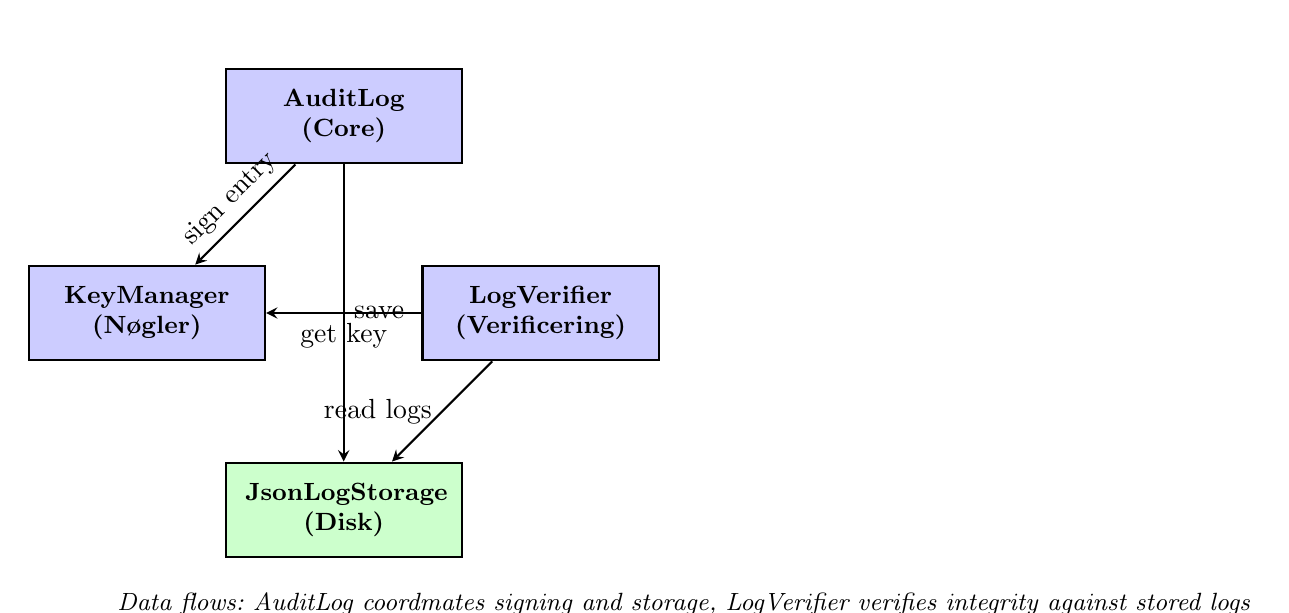
\begin{tikzpicture}[
    component/.style={
        rectangle,
        draw=black,
        fill=blue!20,
        minimum width=3cm,
        minimum height=1.2cm,
        thick,
        font=\small\bfseries
    },
    storage/.style={
        rectangle,
        draw=black,
        fill=green!20,
        minimum width=3cm,
        minimum height=1.2cm,
        thick,
        font=\small\bfseries
    },
    arrow/.style={
        ->,
        thick,
        >=stealth
    }
]

% Components
\node[component] (auditlog) at (3, 5) {\parbox{2.5cm}{\centering AuditLog \\ (Core)}};
\node[component] (keymanager) at (0.5, 2.5) {\parbox{2.5cm}{\centering KeyManager \\ (Nøgler)}};
\node[component] (verifier) at (5.5, 2.5) {\parbox{2.5cm}{\centering LogVerifier \\ (Verificering)}};
\node[storage] (storage) at (3, 0) {\parbox{2.5cm}{\centering JsonLogStorage \\ (Disk)}};

% Arrows
\draw[arrow] (auditlog) -- (keymanager) node[midway, above, sloped, distance=0.3cm] {sign entry};
\draw[arrow] (auditlog) -- (storage) node[midway, right, distance=0.3cm] {save};
\draw[arrow] (verifier) -- (keymanager) node[midway, below, sloped, distance=0.3cm] {get key};
\draw[arrow] (verifier) -- (storage) node[midway, left, distance=0.3cm] {read logs};

% Data flow legend
\node[anchor=west] at (0, -1.2) {
    \small \textit{Data flows: AuditLog coordmates signing and storage, LogVerifier verifies integrity against stored logs}
};

\end{tikzpicture}
\end{center}

\subsection{Komponenter}

\subsubsection{AuditLog (Kerne)}
Hovedklassen som håndterer oprettelse af nye log entries. Den koordinerer med KeyManager for at signere entries og sender dem til JsonLogStorage for persistering. Hver entry linkes til den forrige gennem hash-værdier.

\subsubsection{KeyManager}
Administrerer kryptografiske nøgler og deres versioner. Tillader nøglerotation uden at ødelægge verificering af ældre entries. Holder styr på hvilken nøgleversion hver entry blev signeret med.

\subsubsection{LogVerifier}
Verificerer integriteten af hele log-kæden. Gennemgår hver entry og kontrollerer:
\begin{itemize}
    \item At hash-kæden er intakt (prevHash matcher forrige entry)
    \item At HMAC er gyldig med den korrekte nøgleversion
    \item At ingen entries er slettet eller manipuleret
\end{itemize}

\subsubsection{JsonLogStorage}
Håndterer persistering af log entries til disk i JSON-format. Implementerer append-only principper og giver læseadgang til hele historien.

% ============================================
% DATAMODELLER
% ============================================
\newpage
\section{Datamodeller}

\subsection{Primære Datastrukturer}
[Beskriv datamodeller her]

\subsubsection{Struktur 1}
[Detaljer om struktur 1]

\subsubsection{Struktur 2}
[Detaljer om struktur 2]

% ============================================
% IMPLEMENTERING
% ============================================
\newpage
\section{Implementering}

\subsection{Teknologivalg}
[Beskriv teknologi-valg her]

\subsection{Centrale Funktioner}
[Beskriv hovedfunktioner her]

\subsubsection{Funktion 1}
[Detaljer om funktion 1]

\subsubsection{Funktion 2}
[Detaljer om funktion 2]

\subsection{Lagring og Persistering}
[Beskriv hvordan data lagres her]

% ============================================
% VERIFIKATION OG TEST
% ============================================
\newpage
\section{Verifikation og Test}

\subsection{Test-Strategi}
[Beskriv test-strategi her]

\subsection{Demonstrativ Test}
[Beskriv demo-eksempler her]

% ============================================
% KILDEKODE
% ============================================
\newpage
\section{Kildekode-Oversigt}

\subsection{Vigtige Filer}
\begin{itemize}
    \item \texttt{[Fil 1]} - [Beskrivelse]
    \item \texttt{[Fil 2]} - [Beskrivelse]
    \item \texttt{[Fil 3]} - [Beskrivelse]
\end{itemize}

\subsection{Kodestuktur}
[Beskriv mappestuktur og organisering her]

% ============================================
% KONKLUSION
% ============================================
\newpage
\section{Konklusion}

[Skriv konklusion her]

\end{document}